For clearity, some of the figures in the thesis have been cropped and scaled down. In this appendix, there are large, uncropped versions of those figures.

\begin{figure}[h]
\centering
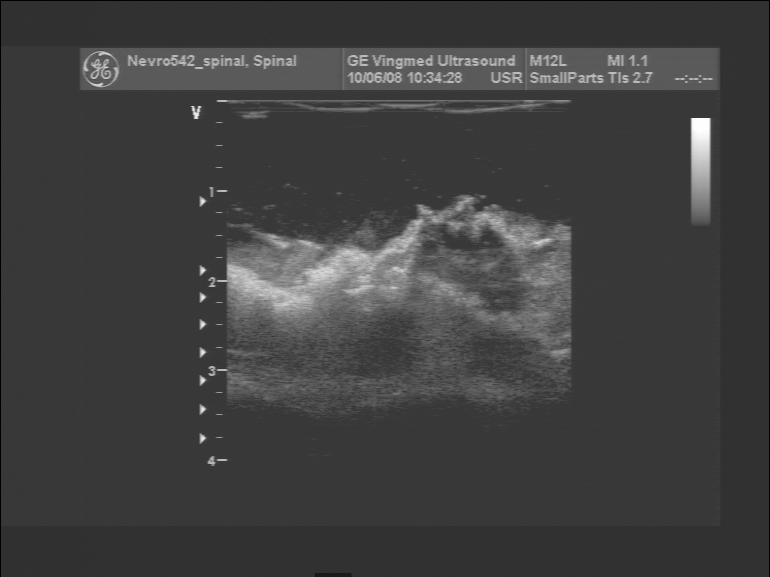
\includegraphics[height=0.45\textheight]{graphics/1.png}
\caption{B-scan number 1/434}
\label{fig:1}
\end{figure}

\begin{figure}[h]
\centering
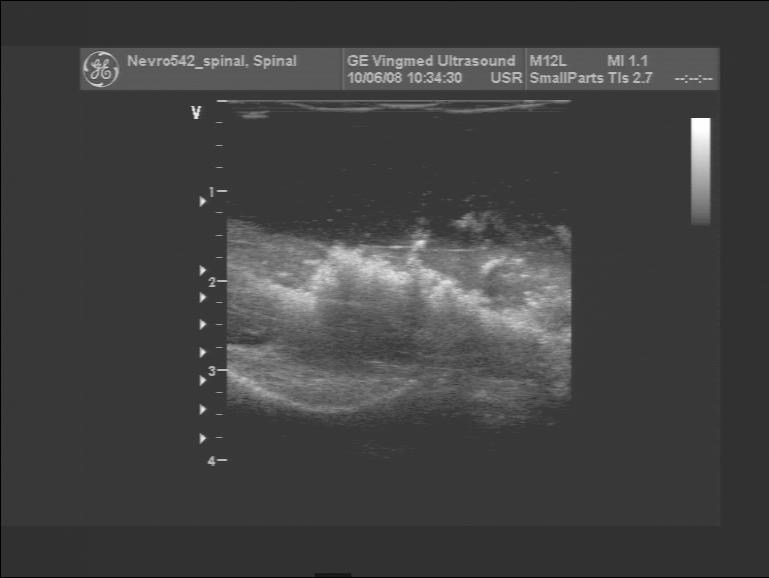
\includegraphics[height=0.45\textheight]{graphics/60.png}
\caption{B-scan number 60/434}
\label{fig:60}
\end{figure}

\begin{figure}[h]
\centering
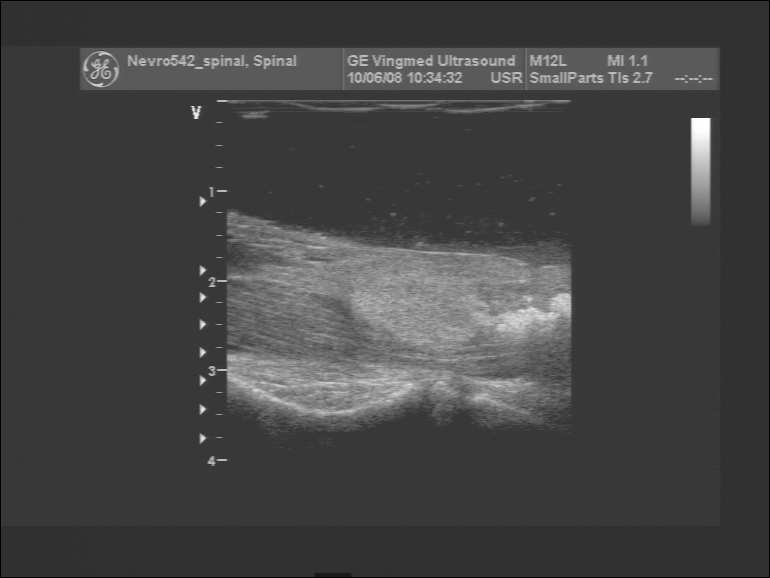
\includegraphics[height=0.45\textheight]{graphics/100.png}
\caption{B-scan number 100/434}
\label{fig:100}
\end{figure}

\begin{figure}[h]
\centering
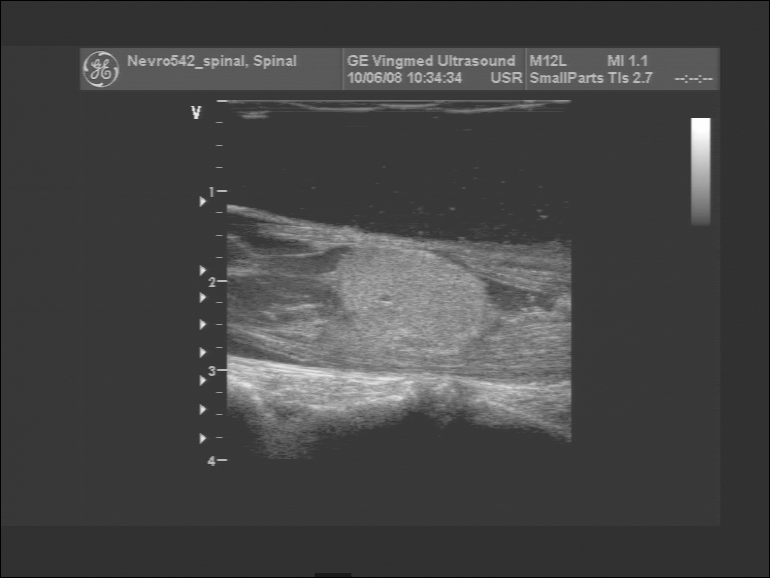
\includegraphics[height=0.45\textheight]{graphics/165.png}
\caption{B-scan number 165/434}
\label{fig:165}
\end{figure}

\begin{figure}[h]
\centering
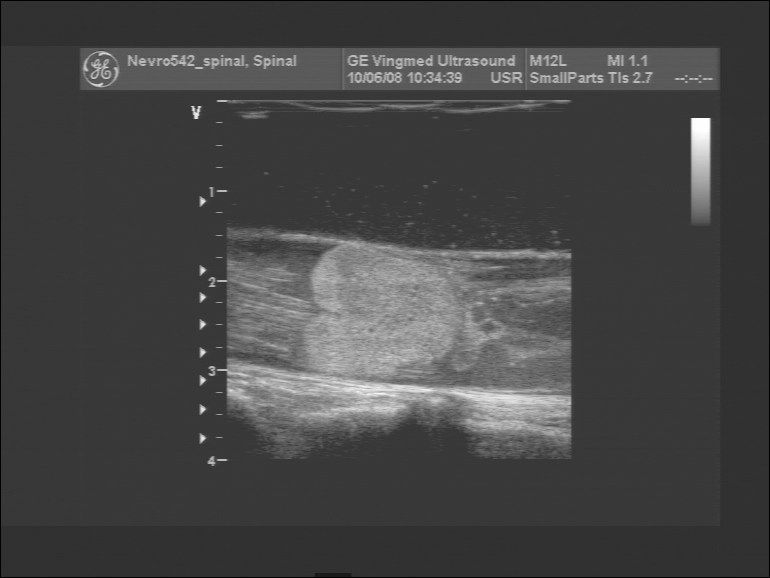
\includegraphics[height=0.45\textheight]{graphics/280.png}
\caption{B-scan number 280/434}
\label{fig:280}
\end{figure}

\begin{figure}[h]
\centering
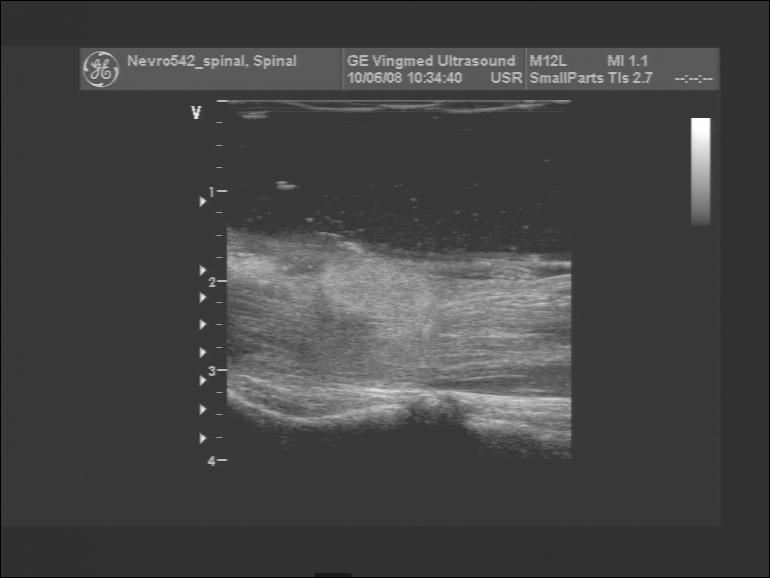
\includegraphics[height=0.45\textheight]{graphics/315.png}
\caption{B-scan number 315/434}
\label{fig:315}
\end{figure}

\begin{figure}[h]
\centering
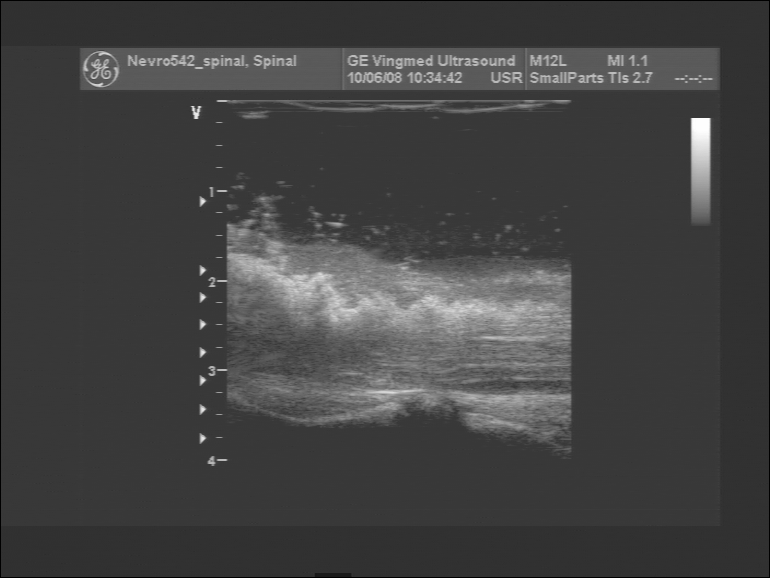
\includegraphics[height=0.45\textheight]{graphics/360.png}
\caption{B-scan number 360/434}
\label{fig:360}
\end{figure}

\begin{figure}[h]
\centering
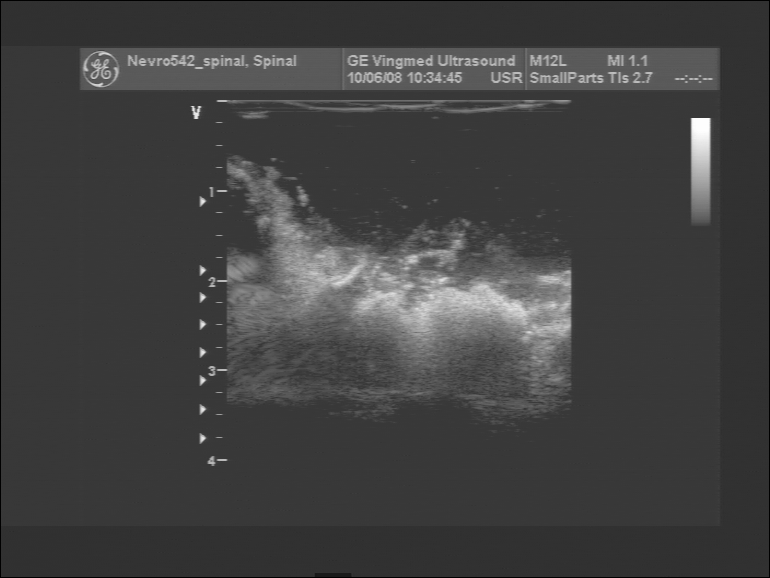
\includegraphics[height=0.45\textheight]{graphics/434.png}
\caption{B-scan number 434/434}
\label{fig:434}
\end{figure}

\begin{figure}[h]
\centering
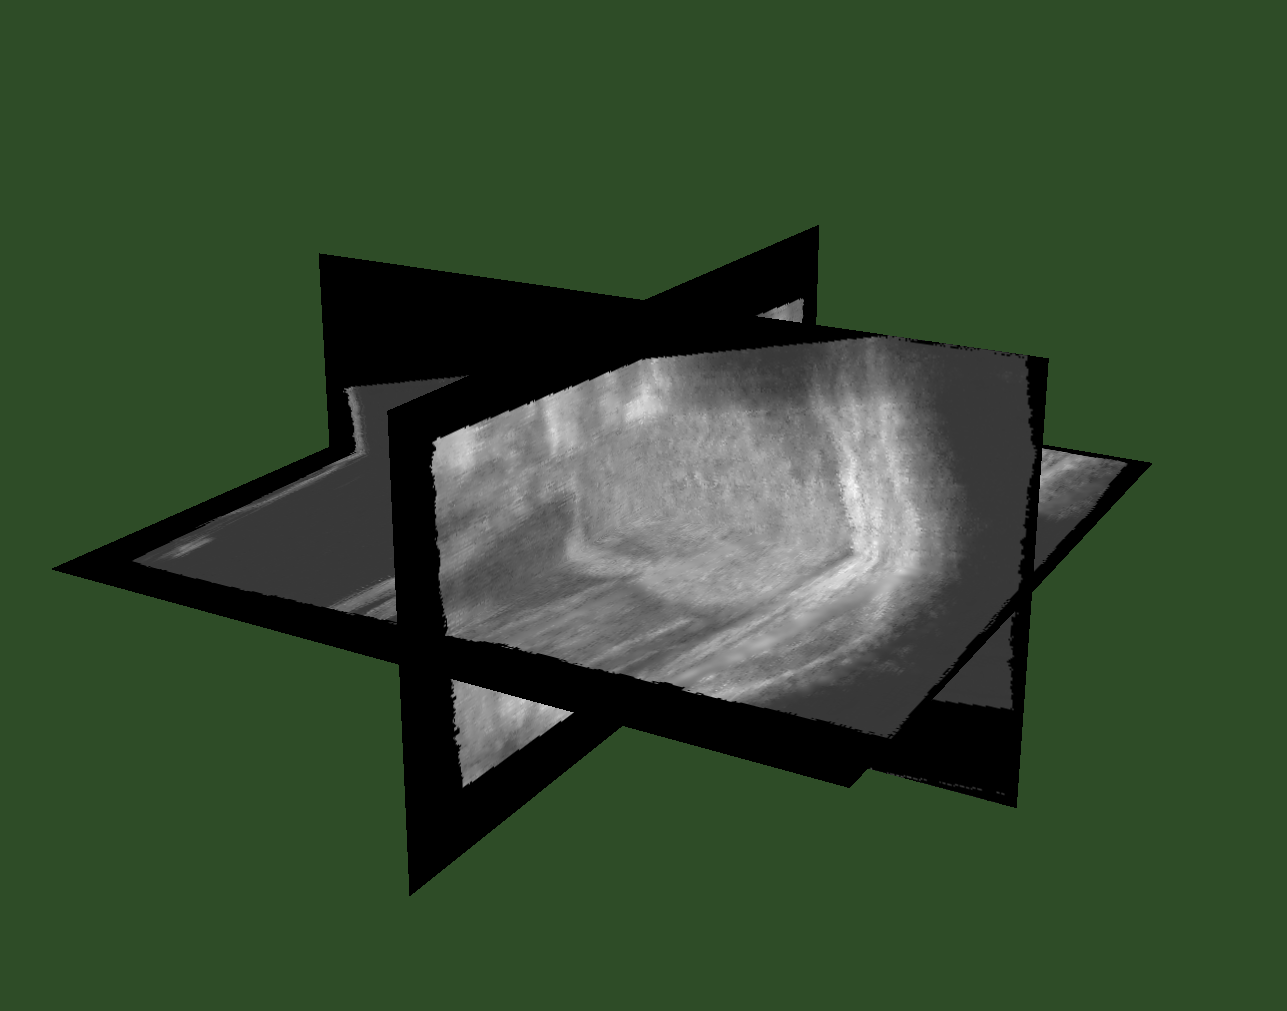
\includegraphics[height=0.45\textheight]{graphics/orthogonal_screen0.png}
\caption{Orthogonal MPR slices screenshot 1}
\label{fig:large_orthogonal_screen0}
\end{figure}

\begin{figure}[h]
\centering
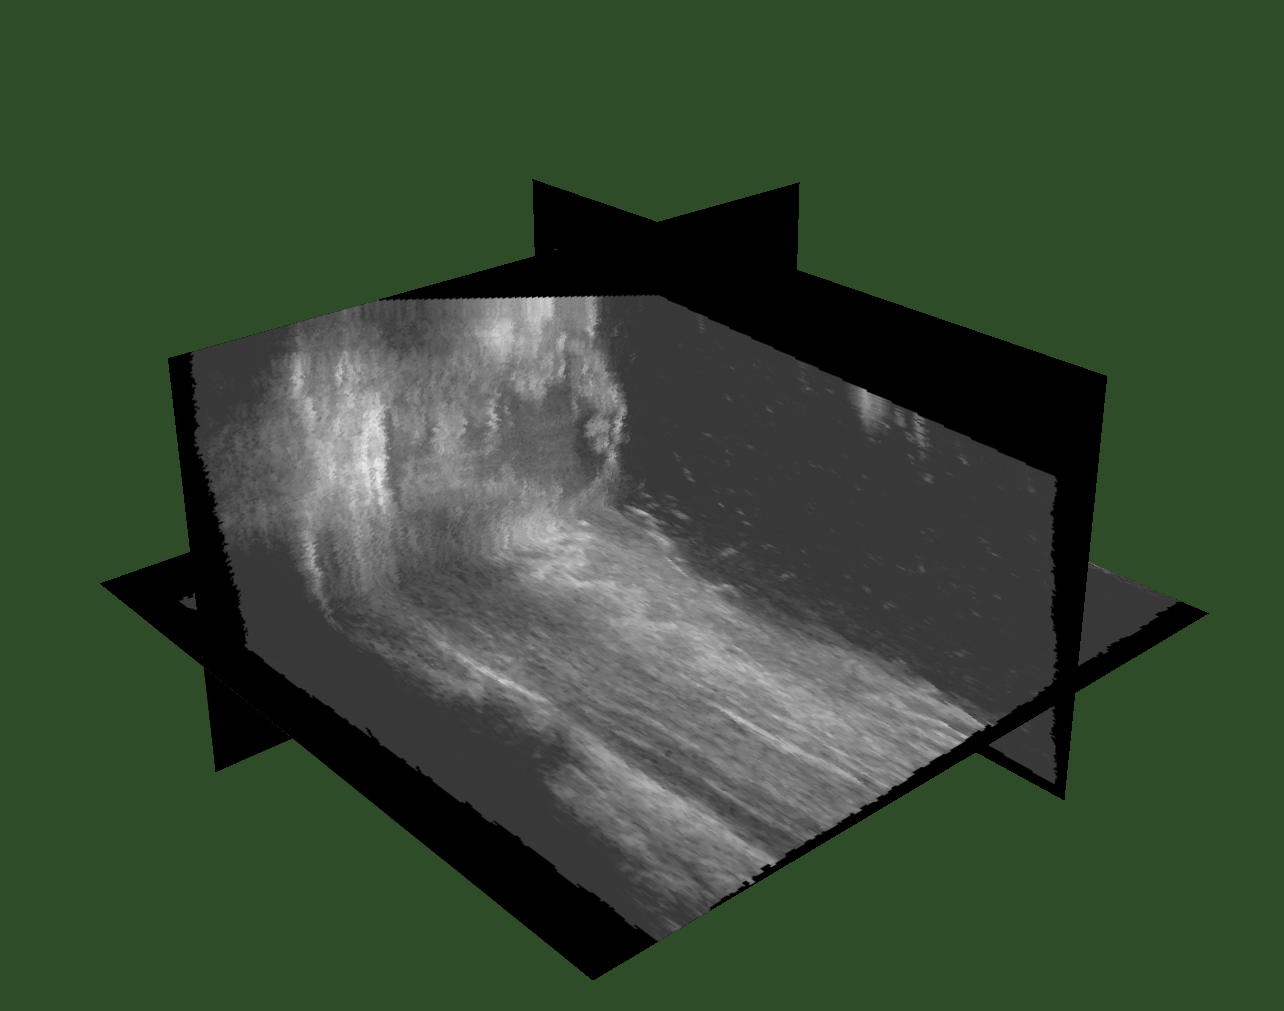
\includegraphics[height=0.45\textheight]{graphics/orthogonal_screen1.png}
\caption{Orthogonal MPR slices screenshot 2}
\label{fig:large_orthogonal_screen1}
\end{figure}

\begin{figure}[h]
\centering
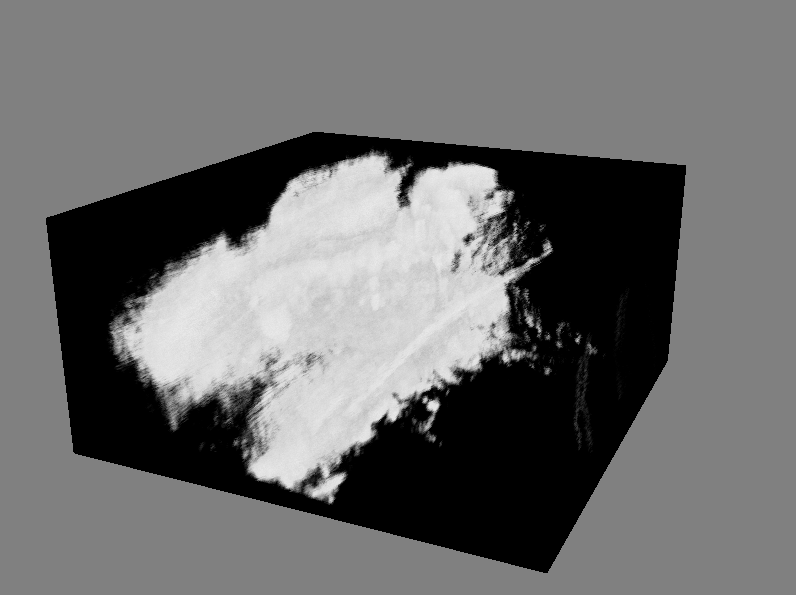
\includegraphics[height=0.45\textheight]{graphics/raycast_screen0.png}
\caption{Ray casting screenshot 1}
\label{fig:large_raycast_screen0}
\end{figure}

\begin{figure}[h]
\centering
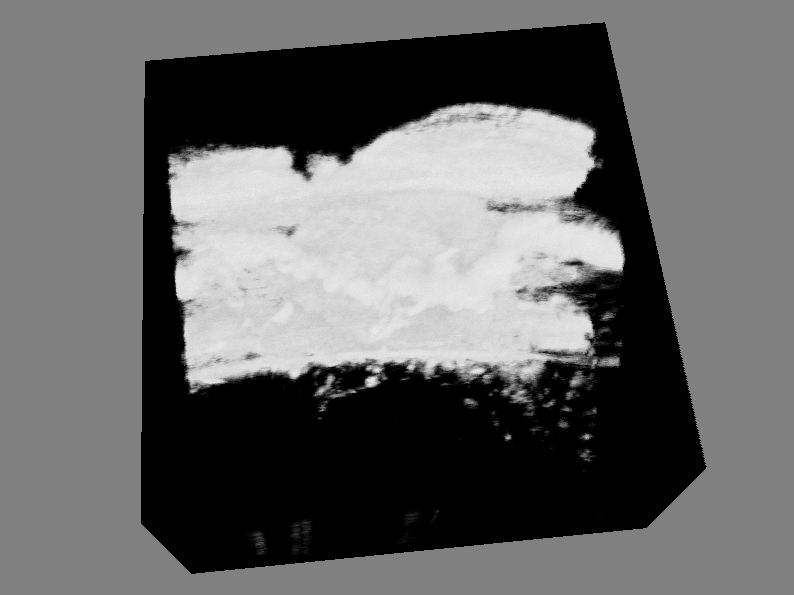
\includegraphics[height=0.45\textheight]{graphics/raycast_screen1.png}
\caption{Ray casting screenshot 2}
\label{fig:large_raycast_screen1}
\end{figure}

%\clearpage

\begin{sidewaysfigure}[h]
\begin{minipage}[b]{0.326\textwidth}
	\centering
	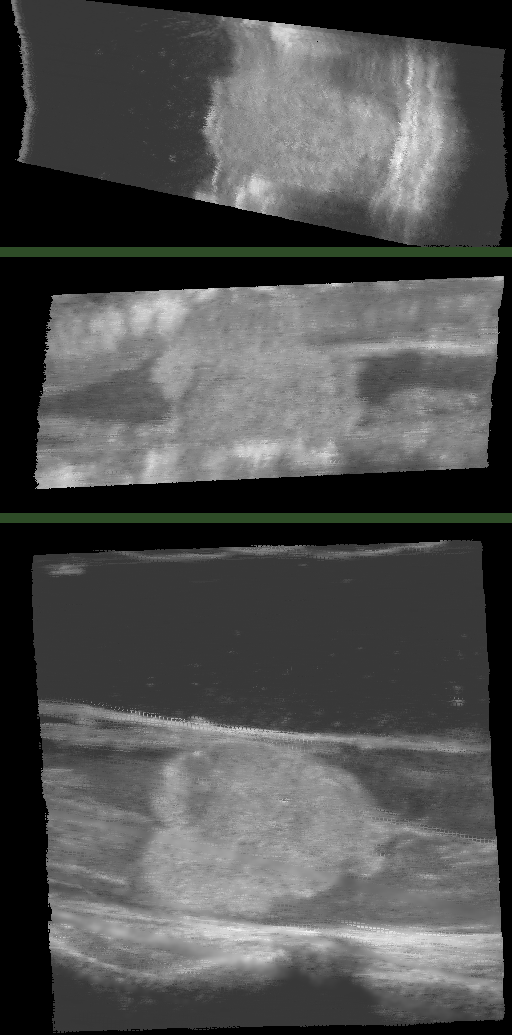
\includegraphics[width=\textwidth]{graphics/large_pnn.png}
	\caption{Volume reconstructed with PNN}
	\label{fig:large_pnn}
\end{minipage}
\hspace{0.01\textwidth}
\begin{minipage}[b]{0.326\textwidth}
	\centering
	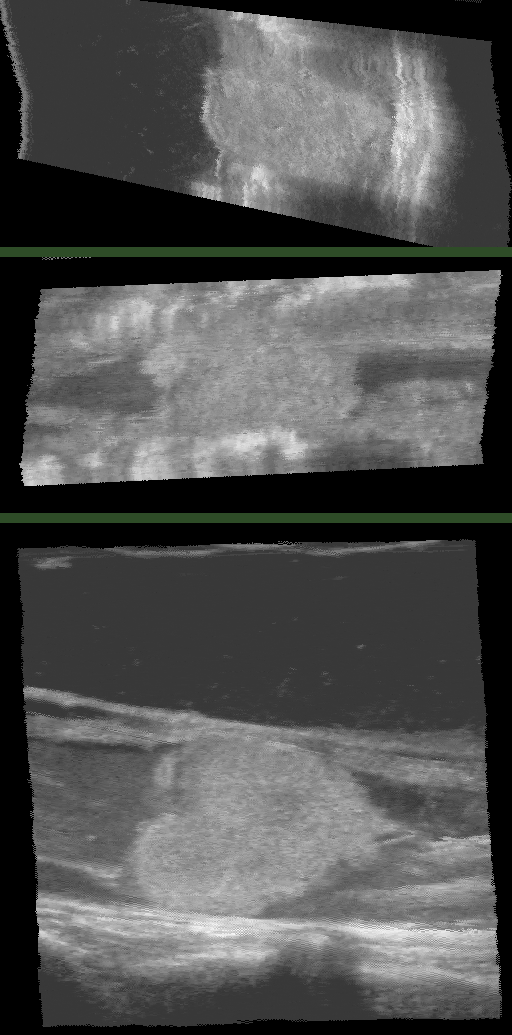
\includegraphics[width=\textwidth]{graphics/large_vnn.png}
	\caption{Volume reconstructed with VNN}
	\label{fig:large_vnn}
\end{minipage}
\hspace{0.01\textwidth}
\begin{minipage}[b]{0.326\textwidth}
	\centering
	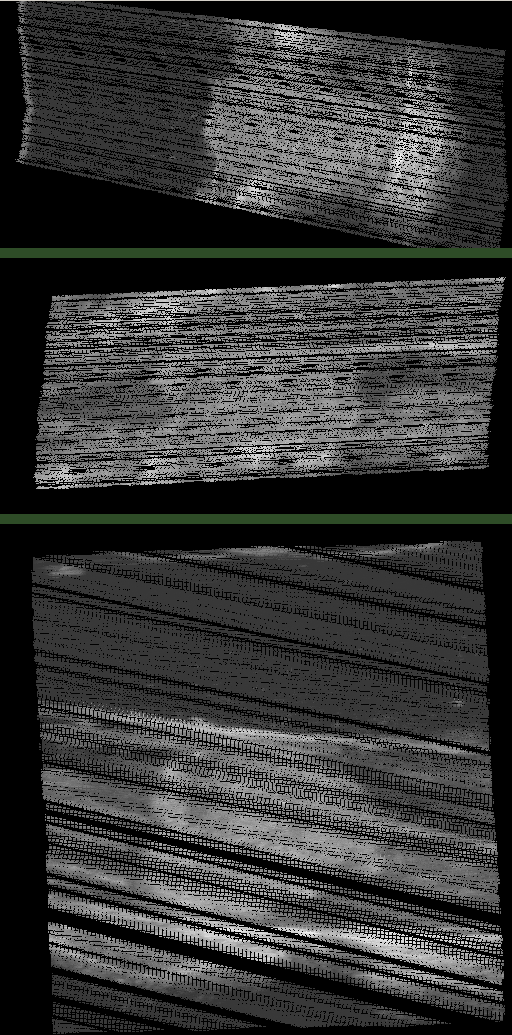
\includegraphics[width=\textwidth]{graphics/large_pnn_holes.png}
	\caption{Volume reconstructed with PNN without hole filling}
	\label{fig:large_pnn_holes}
\end{minipage}
\end{sidewaysfigure}


\begin{sidewaysfigure}[h]
\begin{minipage}[b]{0.326\textwidth}
	\centering
	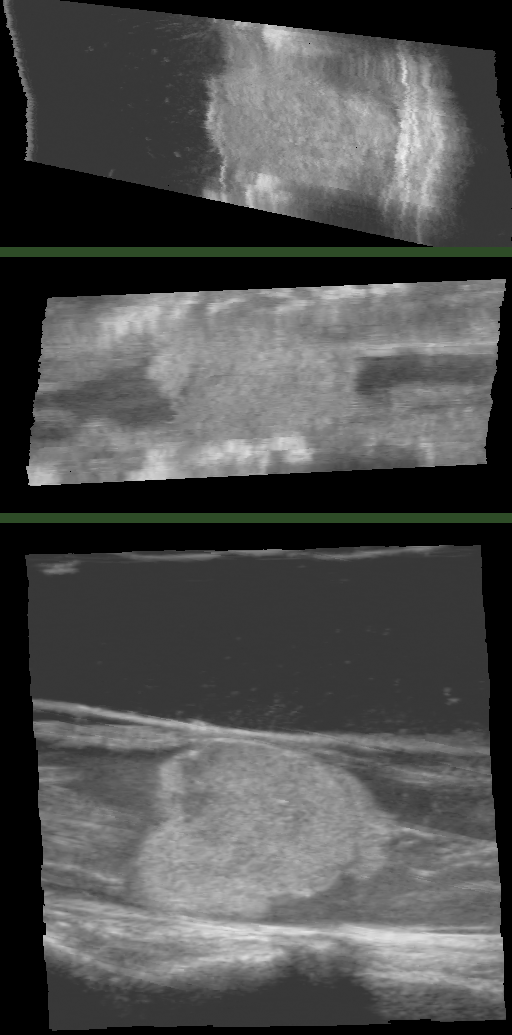
\includegraphics[width=\textwidth]{graphics/large_dwop4.png}
	\caption{Volume reconstructed with $DWOP_4$}
	\label{fig:large_dwop4}
\end{minipage}
\hspace{0.01\textwidth}
\begin{minipage}[b]{0.326\textwidth}
	\centering
	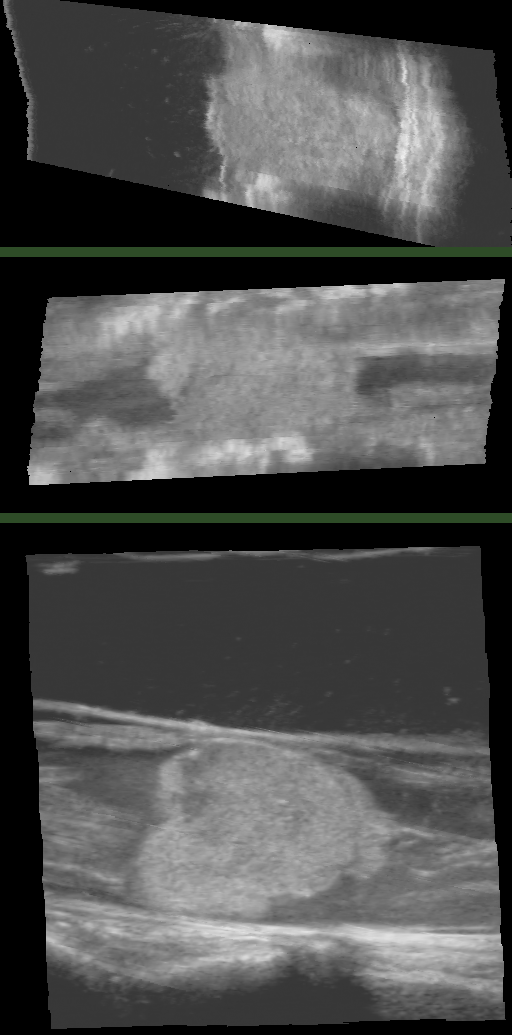
\includegraphics[width=\textwidth]{graphics/large_dwop8.png}
	\caption{Volume reconstructed with $DWOP_8$}
	\label{fig:large_dwop8}
\end{minipage}
\hspace{0.01\textwidth}
\begin{minipage}[b]{0.326\textwidth}
	\centering
	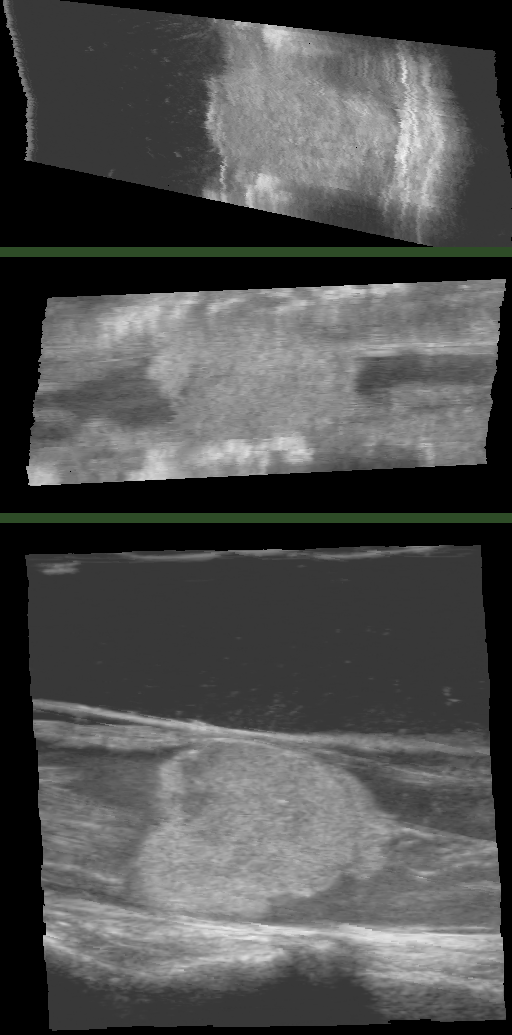
\includegraphics[width=\textwidth]{graphics/large_pt.png}
	\caption{Volume reconstructed with PT}
	\label{fig:large_pt}
\end{minipage}
\end{sidewaysfigure}

\begin{sidewaysfigure}[h]
\begin{minipage}[b]{0.326\textwidth}
	\centering
	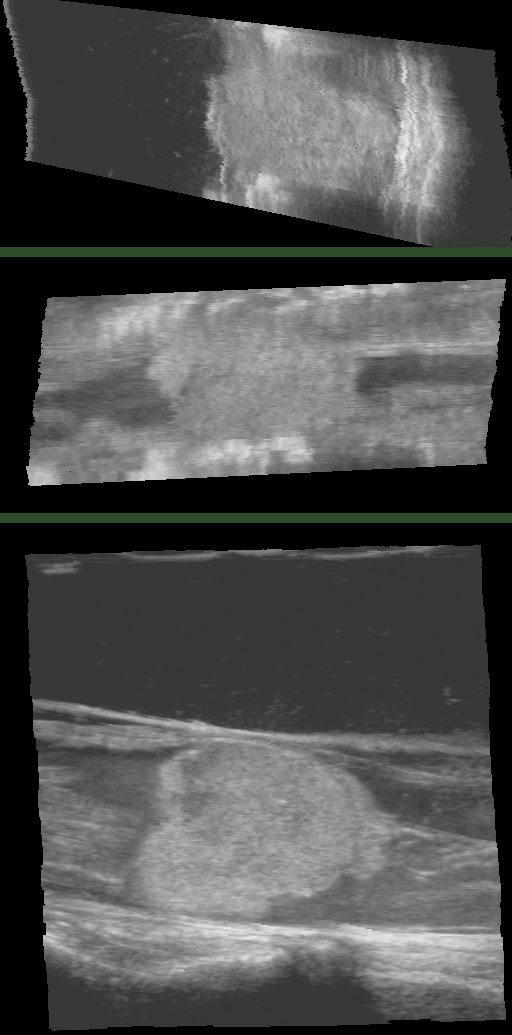
\includegraphics[width=\textwidth]{graphics/large_overwrite.png}
	\caption{Result of $overwrite$ compounding method}
	\label{fig:large_overwrite}
\end{minipage}
\hspace{0.01\textwidth}
\begin{minipage}[b]{0.326\textwidth}
	\centering
	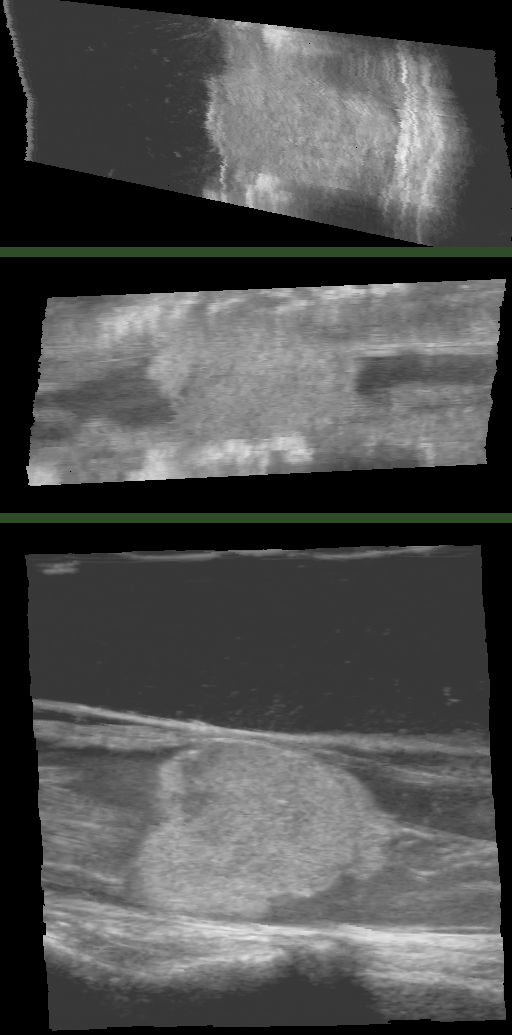
\includegraphics[width=\textwidth]{graphics/large_avg.png}
	\caption{Result of $avg$ compounding method}
	\label{fig:large_avg}
\end{minipage}
\hspace{0.01\textwidth}
\begin{minipage}[b]{0.326\textwidth}
	\centering
	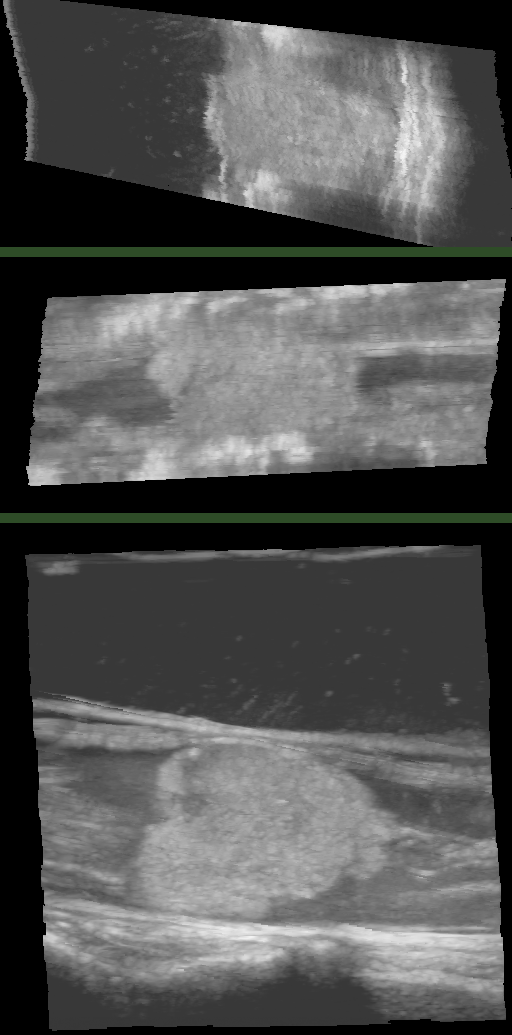
\includegraphics[width=\textwidth]{graphics/large_max.png}
	\caption{Result of $max$ compounding method}
	\label{fig:large_max}
\end{minipage}
\end{sidewaysfigure}

\begin{sidewaysfigure}[h]
\begin{minipage}[b]{0.49\textwidth}
	\centering
	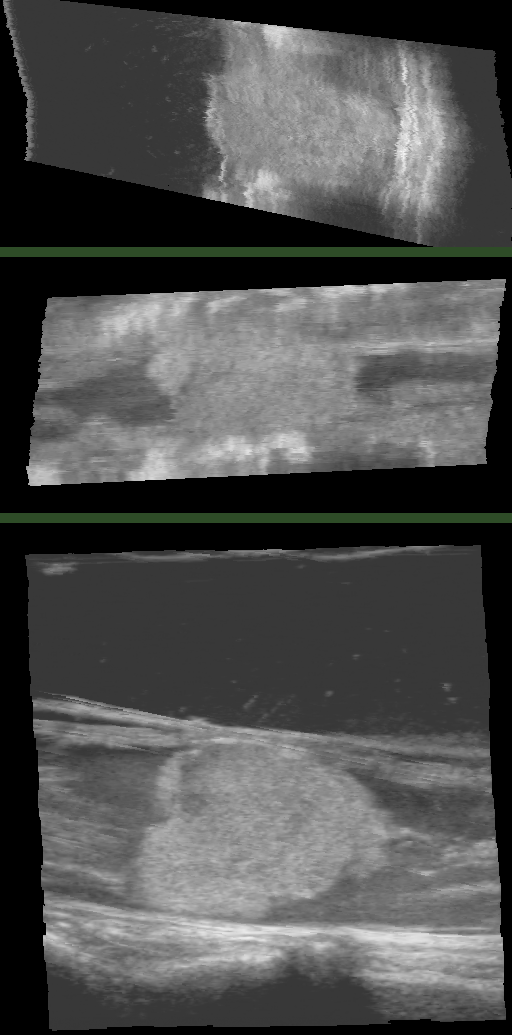
\includegraphics[width=0.652\textwidth]{graphics/large_ifempty.png}
	\caption{Result of $ifempty$ compounding method}
	\label{fig:large_ifempty}
\end{minipage}
\hspace{0.02\textwidth}
\begin{minipage}[b]{0.49\textwidth}
	\centering
	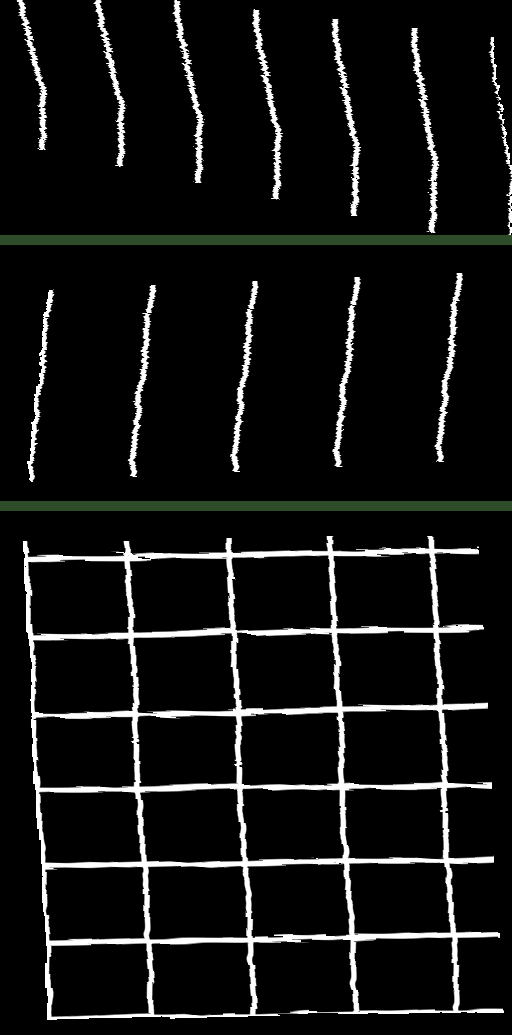
\includegraphics[width=0.652\textwidth]{graphics/large_lines.png}
	\caption{Reconstructed volume of lines with real tracking data}
	\label{fig:large_lines}
\end{minipage}
\end{sidewaysfigure}